\usepackage[utf8]{inputenc}
\usepackage[T1]{fontenc}
\usepackage{mathptmx}
\usepackage[scaled=.90]{helvet}
\usepackage{courier}
\usepackage{caption}
\captionsetup{labelformat=empty,labelsep=none}
\usepackage{verbatim}
\usepackage{hyperref}
\usepackage{listings}
% strikethrough (\sout)
\usepackage{ulem}
\lstset{language=Perl,basicstyle=\normalsize,tabsize=3,showstringspaces=false}

\title{Mobile Shop}
\author[racke]{Stefan Hornburg (Racke)\\  \texttt{racke@linuxia.de}}
\date{Perl::Dancer Conference 2014, Hancock, 9th October 2014}

\begin{document}
\maketitle{}

\begin{frame}
  \titlepage
\end{frame}

\tableofcontents

This presentation is about a mobile shop project for Calevo.

\begin{frame}{Calevo}
\begin{center}
  
\includegraphics{pics/calevo.jpg}
\end{center}
\begin{itemize}
\item Products for riders and horses
\item Since 15 years with Interchange 
\end{itemize}
\end{frame}

Instead of rewriting the old Interchange5 application, we started
to build a Dancer application from scratch.

We are using the same database as for the regular shop though.

Planned release at this end, but it doesn't work out.

The Vary HTTP header should be used to signal caching servers
and help search engine bots to discover mobile-optimized faster.

\begin{frame}{Mobile optimized website}
\begin{itemize}
% Bootstrap
\item Responsive Design
\begin{itemize}
  \item Bootstrap
  \item Foundation
\end{itemize}
\item Dynamically serving different HTML
\begin{itemize}
  \item UserAgent
  \item Vary HTTP header
\end{itemize}
\item Separate Domain
\end{itemize}
\end{frame}

\begin{frame}{Why separate domain}
\begin{itemize}
\item Avoid full rewrite 
\item Focus on the basics
\item Play with modern website
\item Keep existing administration
\end{itemize}
\end{frame}

\begin{frame}{Disadvantages}
\begin{itemize}
\item Reimplementation
\begin{itemize}
\item Payment
\item Prices, Discount
\item Navigation
\end{itemize}
\item Conflicts
\item Maintenance
\end{itemize}
\end{frame}

\section{Showcase}

\begin{frame}{Calevo Mobile}
\begin{itemize}
\item \url{mobile.calevo.com}
\item Coming soon
\end{itemize}
\end{frame}

\subsection{Home}
\begin{frame}[plain]{Home}
\begin{center}
  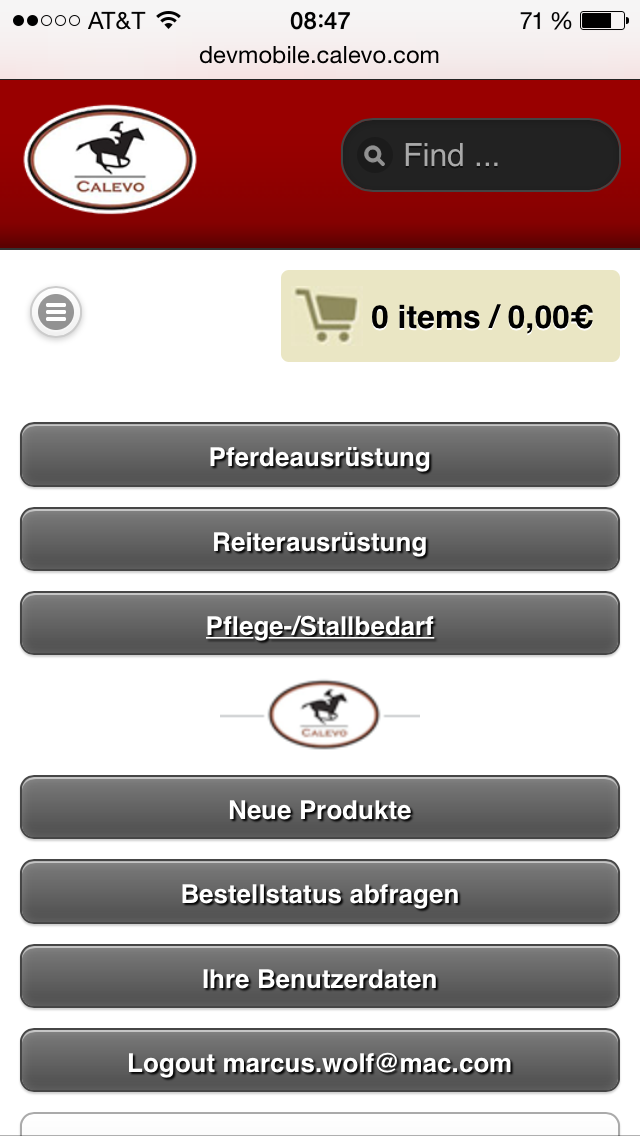
\includegraphics[width=\textwidth,height=1\textheight,keepaspectratio]{pics/home.png}
\end{center}
\end{frame}

\subsection{Category}
\begin{frame}[plain]{Category}
\begin{center}
  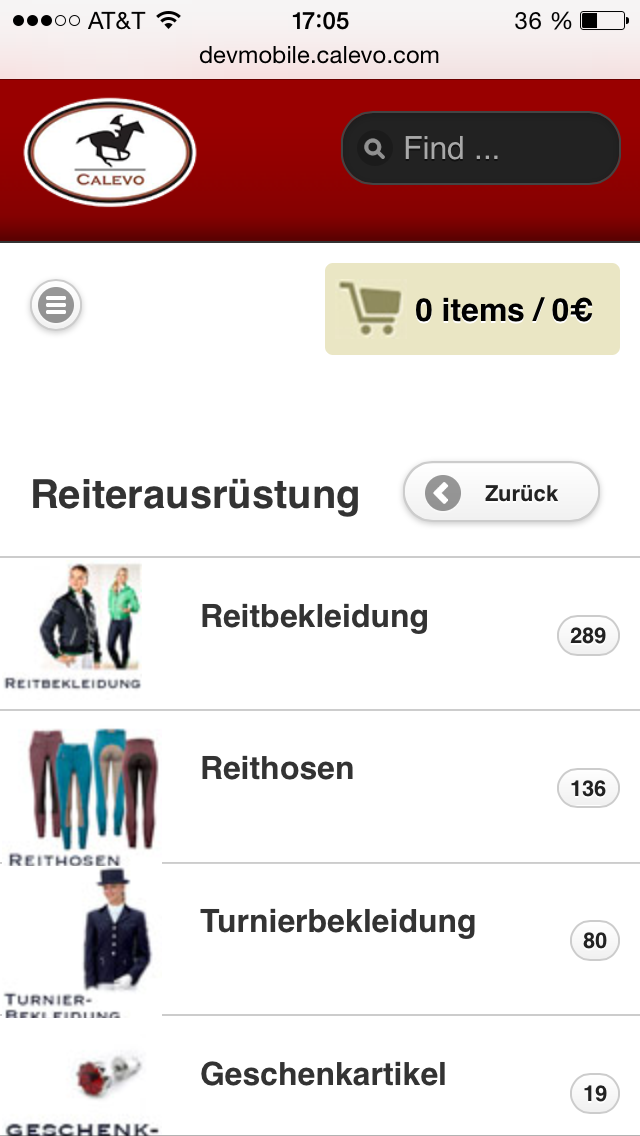
\includegraphics[width=\textwidth,height=1\textheight,keepaspectratio]{pics/category.png}
\end{center}
\end{frame}

\subsection{Cart}
\begin{frame}[plain]{Cart}
\begin{center}
  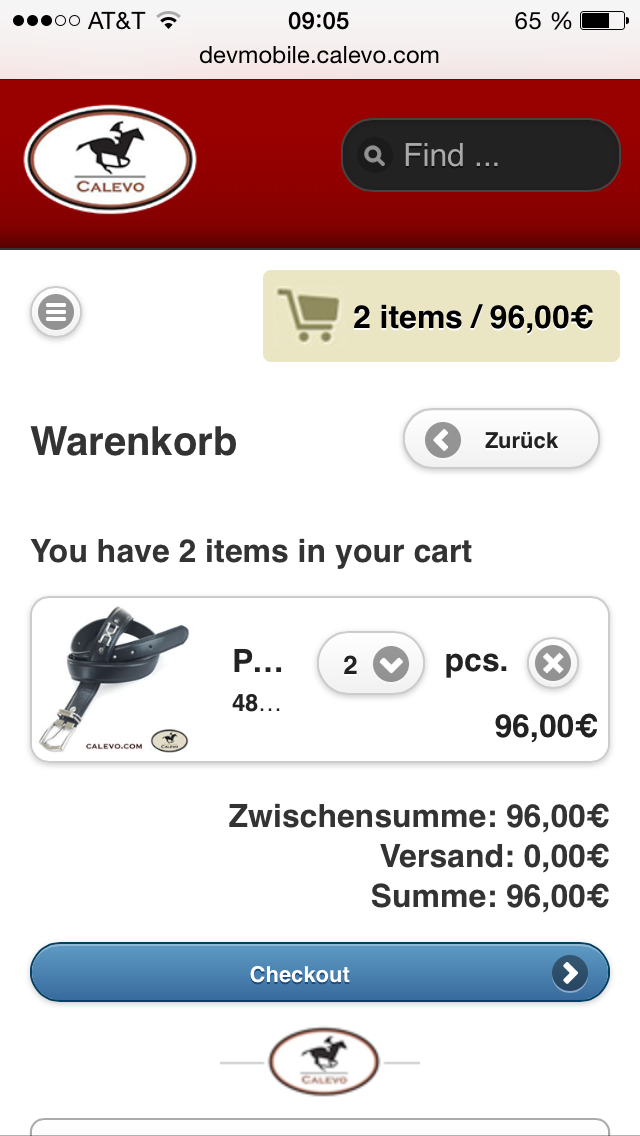
\includegraphics[width=\textwidth,height=1\textheight,keepaspectratio]{pics/cart.png}
\end{center}
\end{frame}

\subsection{Payment}
\begin{frame}[plain]{Payment}
\begin{center}
  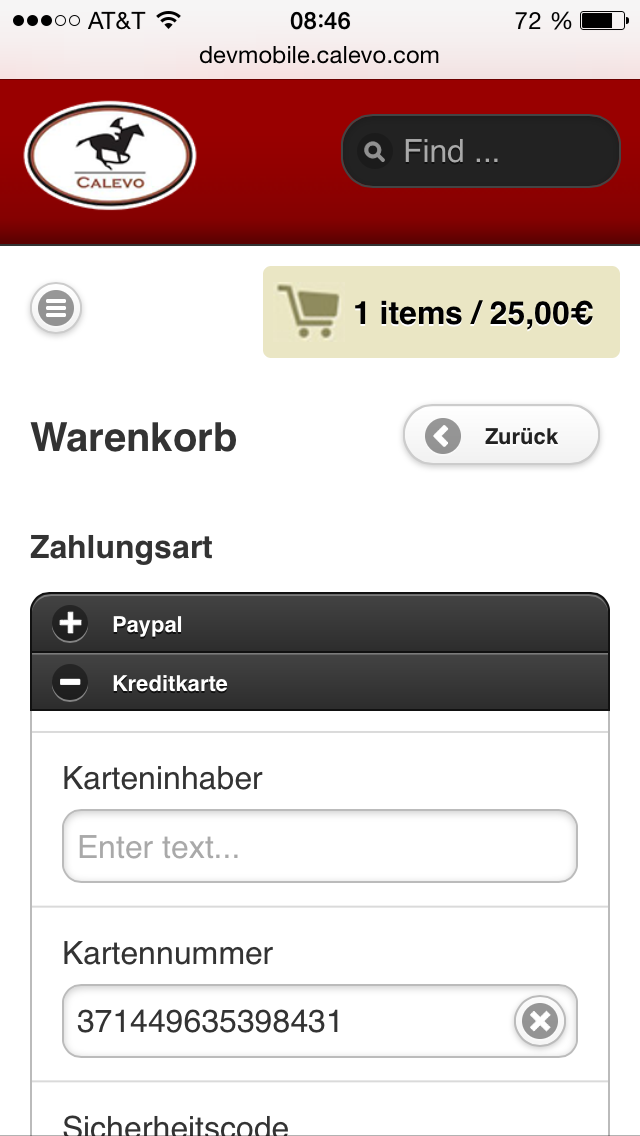
\includegraphics[width=\textwidth,height=1\textheight,keepaspectratio]{pics/payment.png}
\end{center}
\end{frame}

\section{Architecture}
\begin{frame}{Architecture}
\begin{itemize}
\item Dancer
\item Template::Flute
\item DBIx::Class
\item Jquery Mobile
\end{itemize}
\end{frame}

We recommend to use the following if you have a heavily customized
database.

\begin{frame}{Database Schema}
\begin{itemize}
\item Keep existing database
\item Write DBIx::Class schema
\item Clean up database
\end{itemize}
\end{frame}

\section{Features}

% Solr updates

\begin{frame}{Features}
\begin{itemize}
\item Search
\item I18N
\item Payment
\end{itemize}
\end{frame}

\subsection{Search}
\begin{frame}{Search}
\begin{itemize}
\item Solr
\item Ajax Autocomplete
\end{itemize}
\end{frame}

\subsection{I18N}
\begin{frame}{I18N}
\begin{itemize}
\item Autodetect
\begin{itemize}
\item{Location}
\item{Language}
\end{itemize}
\item Translations
\begin{itemize}
\item German
\item English
\item Dutch
\item Swedish
\end{itemize}
\end{itemize}
\end{frame}

\begin{frame}[fragile]{I18N}
\begin{itemize}
\item \verb|products/locale.txt|
\item .po files
\item Translate static text
\end{itemize}
\end{frame}

\begin{frame}[fragile]{I18N with Template::Flute}
\begin{lstlisting}
engines:
  template_flute:
    i18n:
      class: CalevoMobile::Lexicon
      method: try_to_translate
\end{lstlisting}
\end{frame}

\begin{frame}[fragile]{I18N with Template::Flute}
\begin{lstlisting}
package CalevoMobile::Lexicon;

use Moo;
use Dancer ':syntax';
use Dancer::Plugin::SimpleLexicon;

sub try_to_translate {
    my ($self, $string) = @_;
    my $translated = l($string);
    # debug(to_dumper($string));
    return $translated;
}
\end{lstlisting}
\end{frame}

\subsection{Payment}
\begin{frame}{Payment}
\begin{itemize}
\item PayPal
\item IPayment
\item Cash in Advance (Vorkasse)
\end{itemize}
\end{frame}

\subsubsection{PayPal}
\begin{frame}[fragile]{PayPal}
\begin{itemize}
\item Business::PayPal::API::ExpressCheckout
\item CalevoMobile::Routes::PayPal
\end{itemize}
\end{frame}

\begin{frame}[fragile]{PayPal}
\begin{lstlisting}
package CalevoMobile::Routes::PayPal;
prefix '/paypal';

# Retrieve a token and send user to PayPal
post '/setrequest' => sub { 
    .. 
    redirect $paypal_url;
};

# Payment response from PayPal
get '/getrequest' => sub { .. };

prefix undef;
\end{lstlisting}
\end{frame}

\subsubsection{IPayment}
\begin{frame}[fragile]{IPayment}
\begin{itemize}
\item Business::OnlinePayment::IPayment
\item Silent CGI
\end{itemize}
\end{frame}


\section{Conclusion}

\subsection{Slides}

\begin{frame}{Slides}
Slides:
\url{http://www.linuxia.de/talks/perldancer2014/mobileshop-en-beamer.pdf}
\end{frame}


\end{document}

%%% Local Variables: 
%%% mode: latex
%%% TeX-master: t
%%% End: 
